\graphicspath{{./figures/}}
\chapter*{Appendix}
\addcontentsline{toc}{chapter}{Appendix}
\renewcommand{\thesection}{\Alph{section}}

\section{Drone}
\label{sec:appendix_drone}
\begin{figure}[htbp]
    \centering
    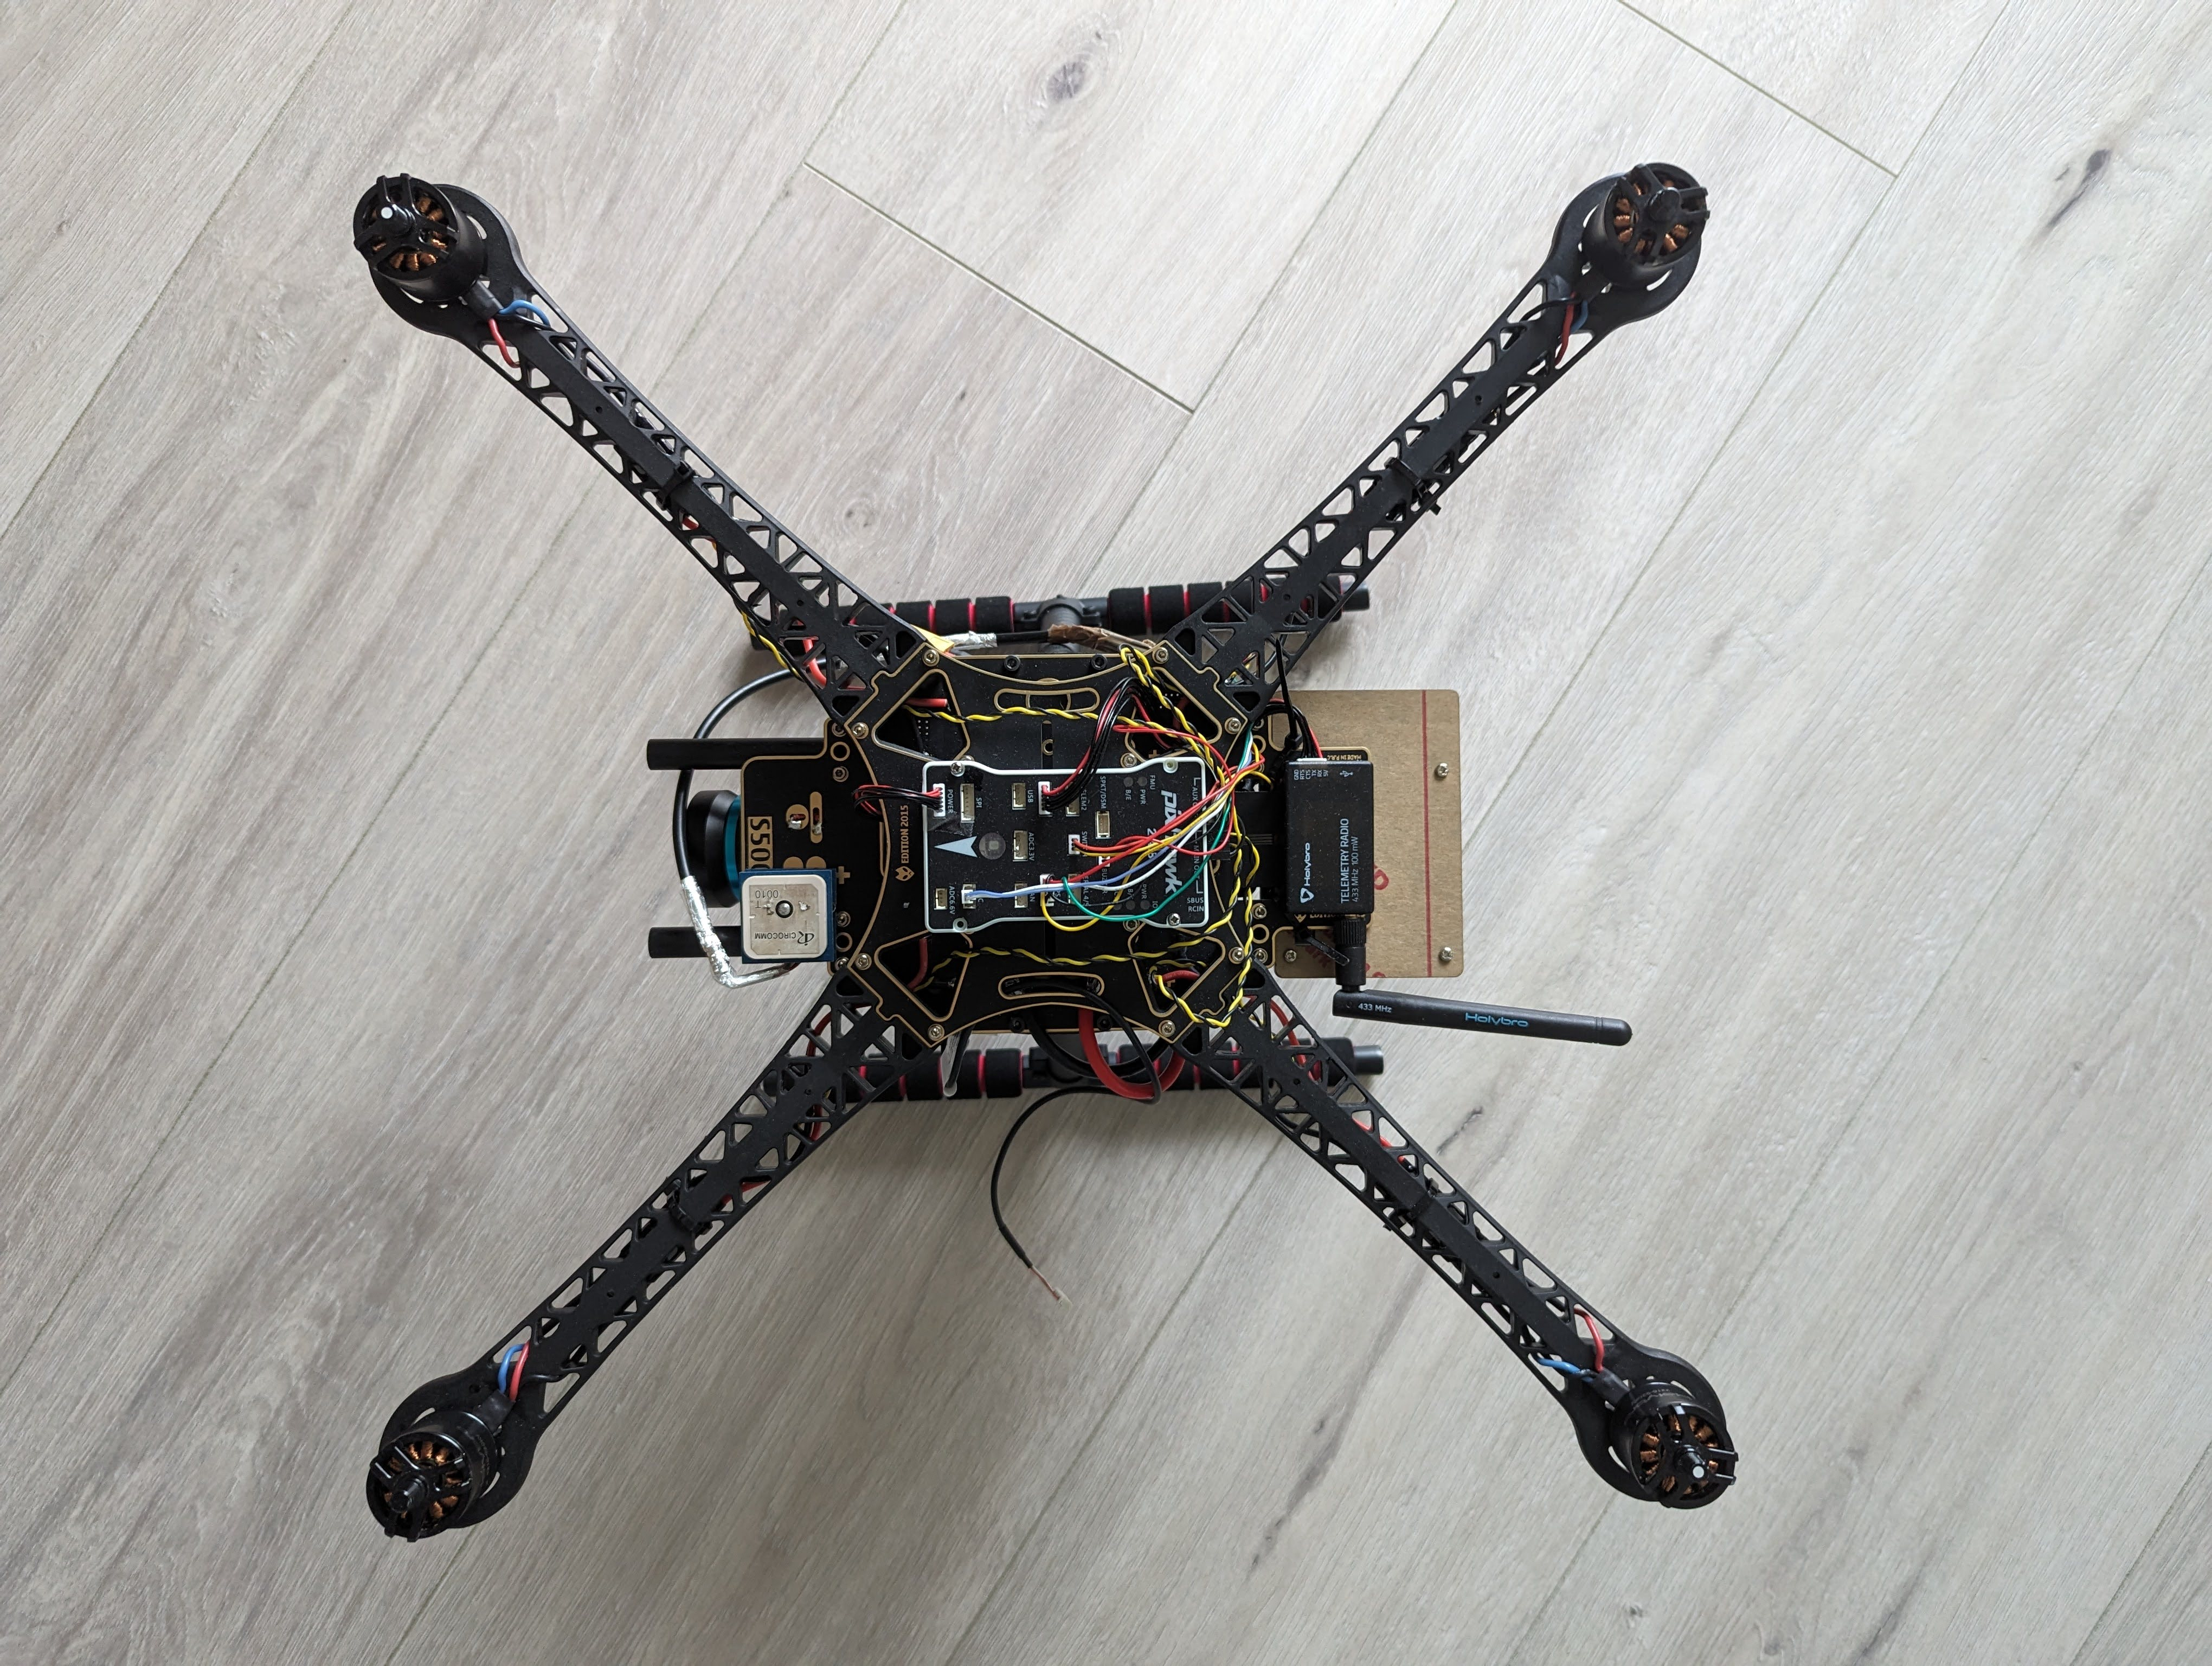
\includegraphics[width=0.4\textwidth]{drone_fully_top.jpg}
    \caption[Fully equipped drone]{Fully equipped drone - Top view.\\
    The PixHawk flight controller is on top of the drone.}
\end{figure}

\begin{figure}[htbp]
    \centering
    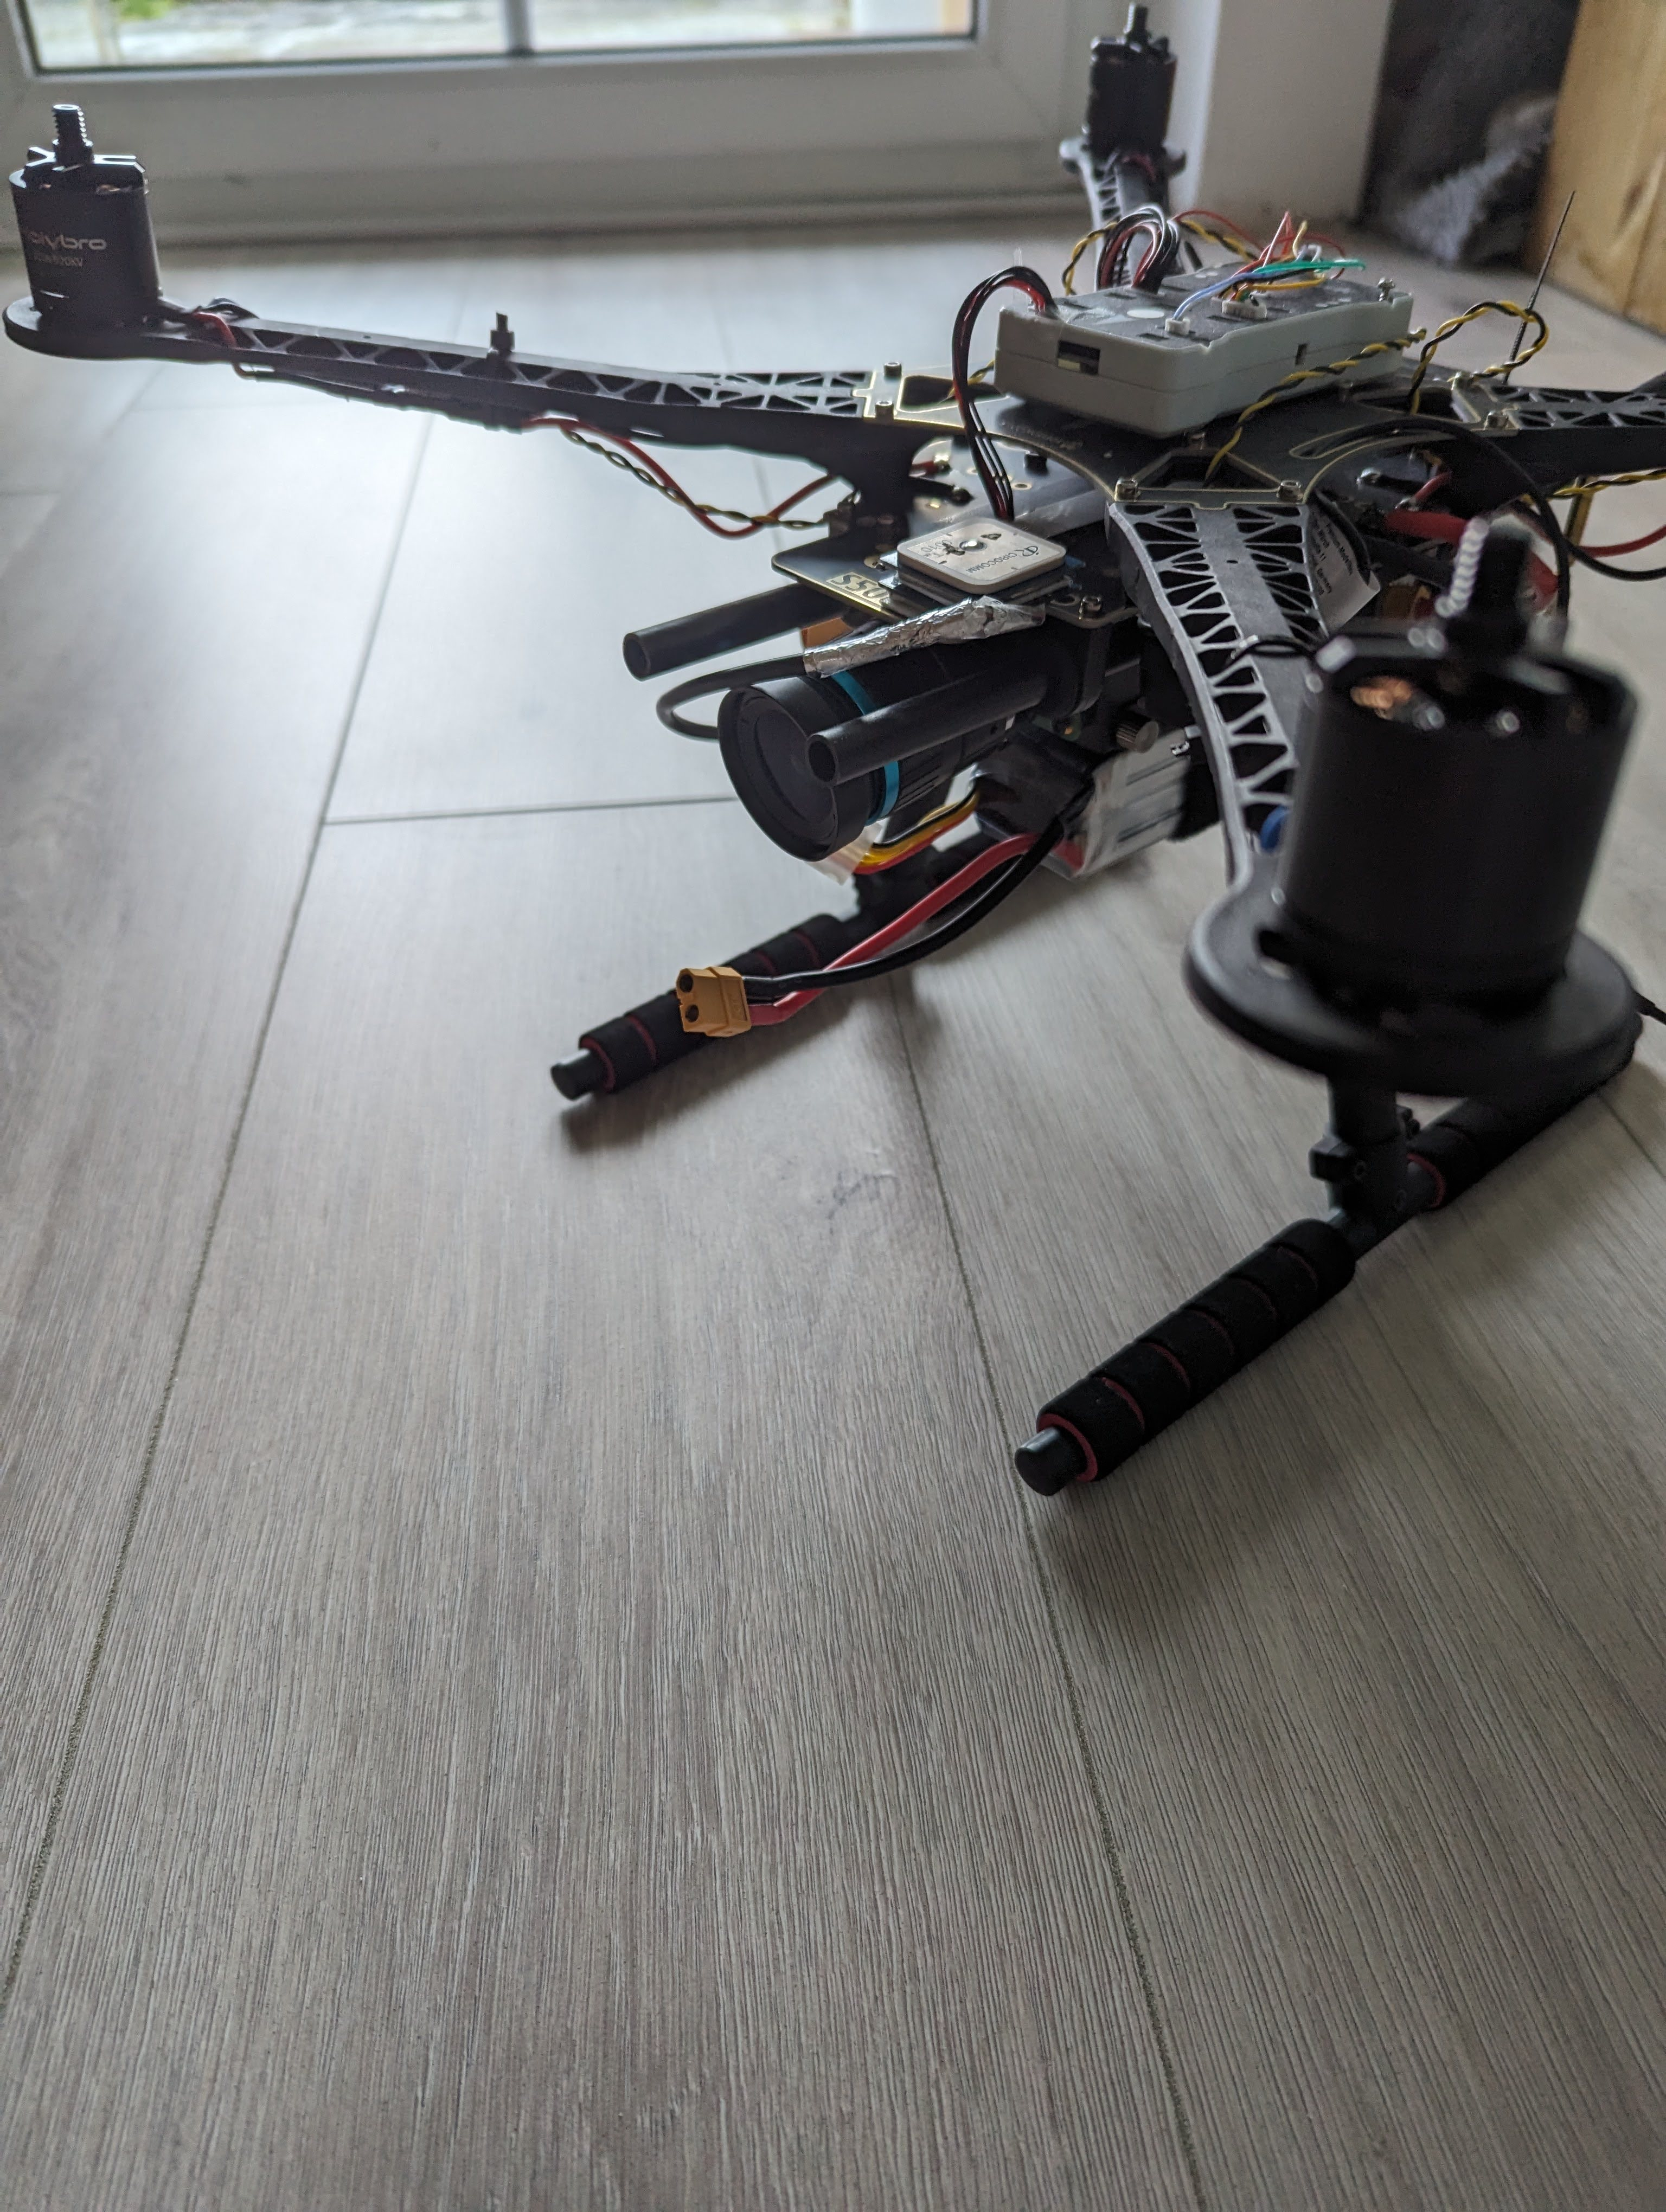
\includegraphics[width=0.4\textwidth]{drone_cam.jpg}
    \caption[Drone with camera]{Drone with a RaspberryPi camera mounted.\\}
\end{figure}
\FloatBarrier
\newpage

\section{Analysis module overview}
\label{sec:appendix_ljanalizer}

The long-jump analysis is implemented as own python module \texttt{ljanalyzer}
with several sub-modules.
The module's structure is showed in the following:
\begin{figure}[h!]
    \centering
    \scalebox{1.2}{ % Adjust the scaling factor as needed
    \centering
        \begin{minipage}{1.0\textwidth}
            \dirtree{%
            .1 ljanalizer.
            .2 Frame.
            .2 Video.
            .2 Posedetector.
            .2 Framebuffer.
            .2 Evaluation.
            .2 Parameterfile.
        }
        \end{minipage}
    }
    \caption[Python analysis module overview]{Python long jump analysis module
    overview.}
    \label{fig:appendix_ljanalizer_overview}
\end{figure}
\FloatBarrier
\noindent As the frame and video sub-module are most important in this work,
both class diagrams are shown in the following:
\begin{figure}[htpb]
    \centering
    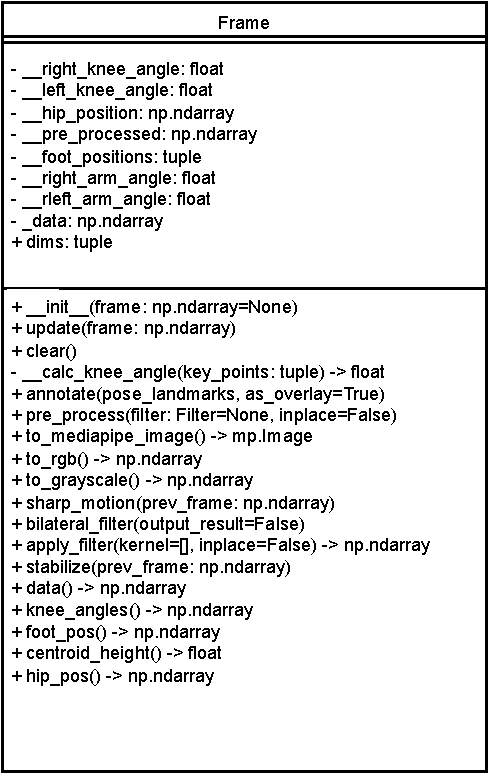
\includegraphics[scale=0.9]{frame_class.pdf}
    \caption[Frame class diagram]{Frame class diagram}
    \label{fig:appendix_frame_class}
\end{figure}

\begin{figure}[htpb]
    \centering
    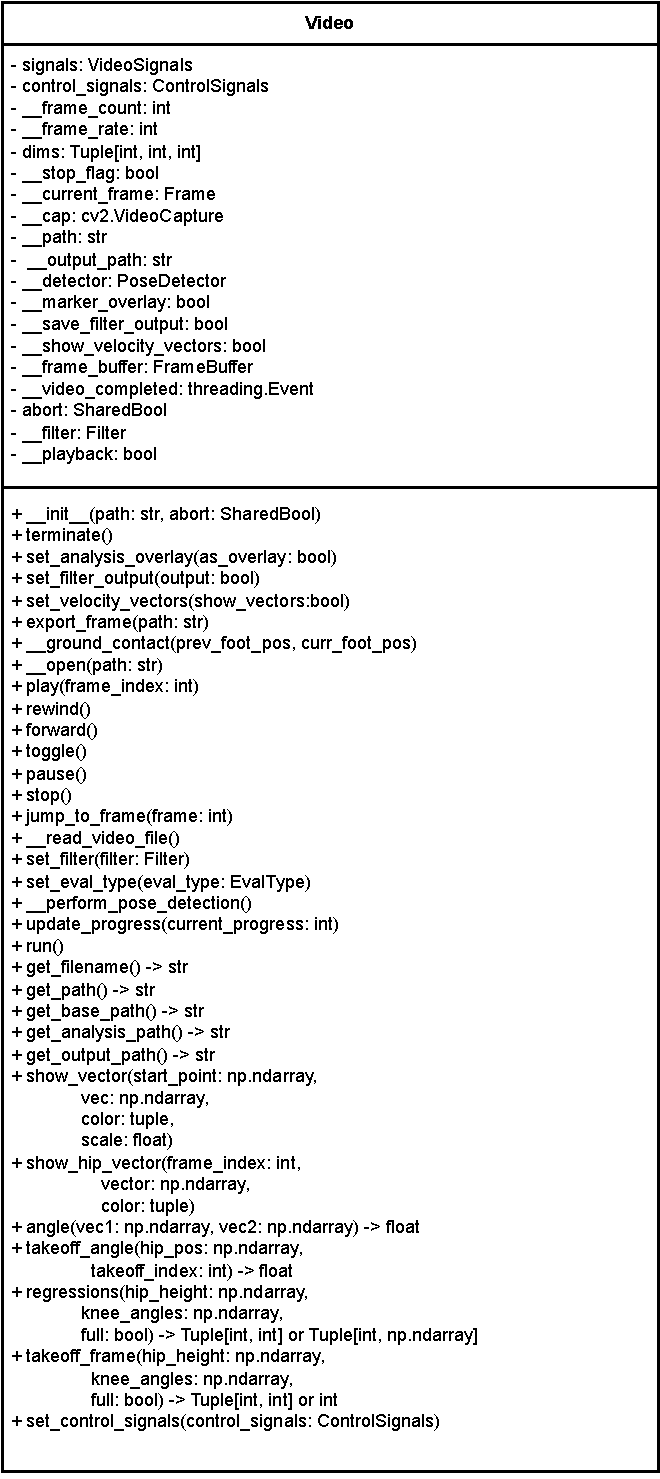
\includegraphics[scale=0.8]{video_class.pdf}
    \caption[Video class diagram]{Video class diagram}
    \label{fig:appendix_video_class}
\end{figure}

\newpage

\section{Live-Stream video visualization}
\label{sec:appendix_livestream}
\begin{figure}[htpb]
    \centering
    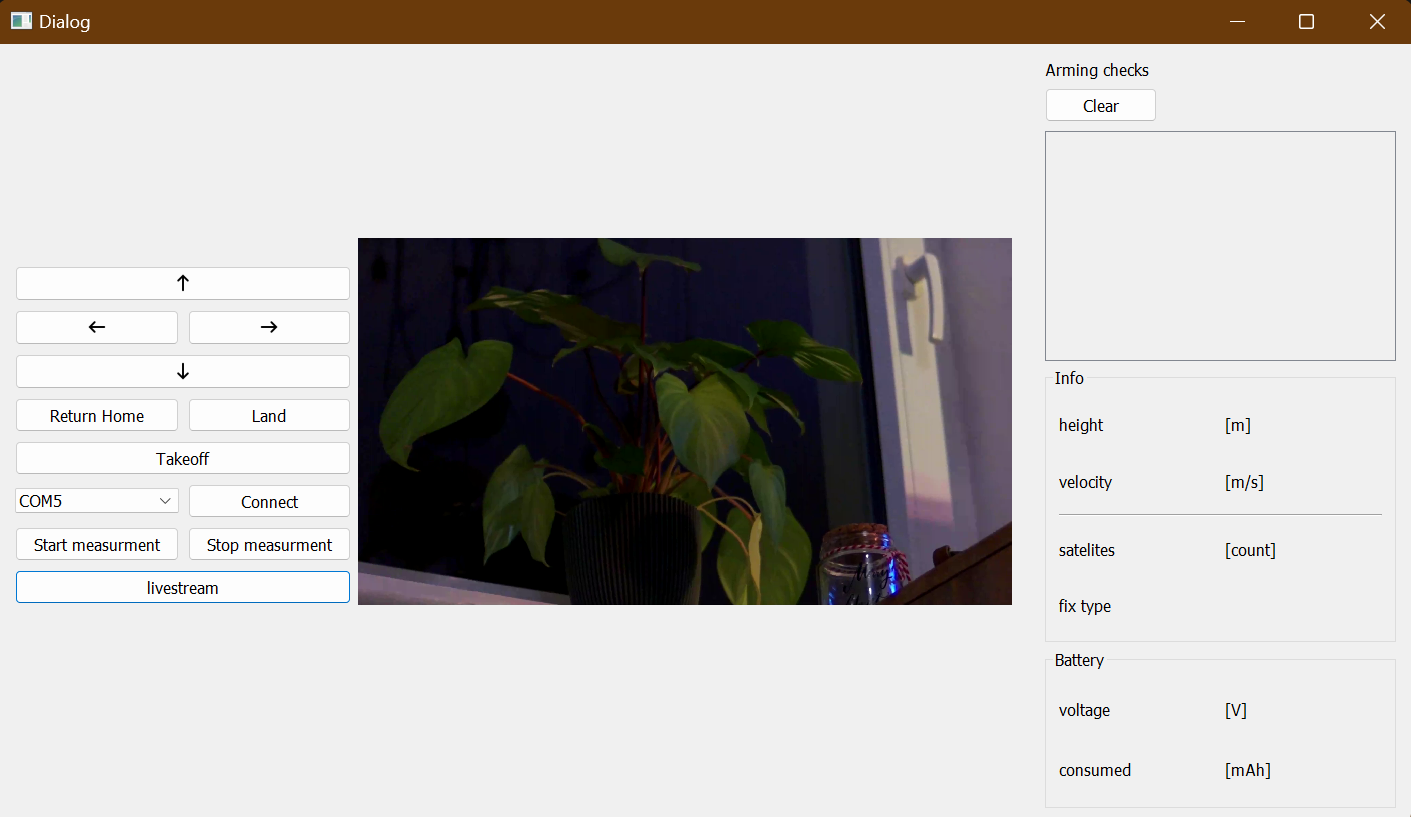
\includegraphics[scale=0.5]{drone_control_panel_live_stream.png}
    \caption[Video Live-stream visualization]{Video Live-stream visualization
    inside the control panel.}
    \label{fig:4_control_panel_live_stream}
\end{figure}
